\section{Theoretical Background}\label{sec:basics}
This section gives an overview of the task that is used within this work (§\ref{sec:basics_nli}) and relevant datasets regarding this task (§\ref{sec:basics_datasets}).
\subsection{Natural Language Inference}\label{sec:basics_nli}
\ac{NLI} \citep{bowman2015large} deals with the problem to identify, whether one piece of natural text, namely the \textit{hypothesis}, can be inferred from another piece of text, namely the \textit{premise}. The hypothesis $h$ is said to be entailed by the premise $p$ if a human reader would conclude that the hypothesis is true, given the fact that the premise is true. Therefore it differes from strict logical inference. While in \ac{NLI} a high plausability for the premise to imply the hyothesis, based on the human judgement, is sufficient, the latter one strives to achieve certainity \citep{dagan2009recognizing}. \ac{NLI} essentially breaks down to an alignment problem \citep{maccartney2008phrase}. Given the sentence pair
\begin{center}
\begin{tabular}{rl}
\textbf{Premise:} & \textit{Donald Trump is eating his cheeseburger in his bedroom.} \\
\textbf{Hypothesis:} & \textit{The president of the United States is snacking a cheeseburger in the White House.} 
\end{tabular}
\end{center}
the model is required to correctly align \textit{Donald Trump} with \textit{The president of the United States}, \textit{eating} with \textit{snacking} and have information that his \textit{bedroom} is within the \textit{White House}. Here it can be seen, how the system would not only need to cope with different ways of expressing the same meaning, due to the nature of language, but also is required to access and process factual information, that is commonly known to an average human. 
\newline
\subsubsection*{Relatedness to other NLP tasks}
While \ac{NLI} clearly is central to reasoning capabilities, it is very fundamental and applicable to a large variety of \ac{NLP} as the ability to recognize textual entailment is a fundamental and necessary problem towards real \ac{NLU} \citep{maccartney2007natural,bos2005recognising}. Many \ac{NLP} applications such as \ac{QA}, Summarization \ac{IE} implicitly depend on this ability, as the huge variability of possible expressions for the same meaning it is a core phenomen of natural language \citep{dagan2009recognizing}. All three tasks require the model to infer that the target meaning of interest can be inferred from any other variant of textual expression. For \ac{QA} it is the identification of a correct answer, for summarization, the complete summary needs to be implied by the original text and similarily, while redundant sentences expressing the same meaning should be ommited. Similarily \ac{IE}, especially if using multiple documents, needs to infer, whether two variants of text contain the same information. Even simple paraphrasing can be broken down to a lexical inference problem with mutual entailment between $p$ and $h$. As end applications for \ac{NLP} in addition to \ac{NLU} need to solve another complicated machine-learning task it is hard to compare and directly improve their \ac{NLU} capabilities. Thus, one of the main purposes of \ac{NLI}, being a very basic problem towards \ac{NLU}, serves a a benchmark  with any improvements helping a large variety of high level tasks \citep{williams2017broad,cooper1996using,bos2005recognising,dagan2006pascal}. 

\subsection{Lexical Semantic Relations}\label{sec:word_relations}
\mx{TODO: lexical inference \citep{shwartz2015learning} and being the semantic relation between two terms (bi/unidirectional)}
Lexical relations describe the relationship between words\footnote{While there is no single definition for \textit{word}, we refer assume a single word to have the same surface form and the same lemma.} whereas \textit{Lexical Semantic Relations} specifically indicate relations referring to the meaning of the word. \citep{murphy2003semantic} and have shown to be helpful for detecting lexical inferences \citep{dagan2009recognizing}. We define the following relations based on those of \cite{Jurafsky2008May}. One key characteristic of natural language is ambiguity, tht is also present in lexical semantics as words may have several meanings or \textit{senses}\footnote{The phenomen of words having multiple senses is called \textit{homonymy}, if both senses show indicate no relation but share the surface form like ``bank'' (financial institution) and ``bank'' (sloping mound). If those senses are semantically related like ``milk'' (take milk from female mammals) and ``milk'' (like cow's milk), the relationship is called \textit{polysemy} \citep{Jurafsky2008May}}. To deal with this phenomene, lexical semantic relations are defined between senses rather than words. For the sake of simplicity for the most part we follow a naive approach in the following chapters of assuming the most dominant sense of a word, when referring to it. Specifically we define \textit{Synonymy}, \textit{Antonomy}, \textit{Hypernomy} and \textit{Holonomy}, the latter two relations are visualized\footnote{This is for illustration purposes only and we only added some relevant relations between the entities, more relation are possible. For instance, the holonym relationship would of course hold between \textit{head} and any other \textit{animal}.} in Figure \ref{fig:lexical_resources}.
\begin{figure}[tph!]
\centering
	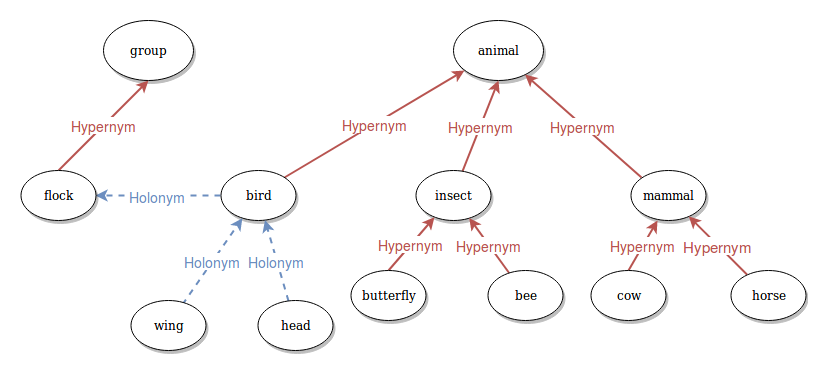
\includegraphics[totalheight=7cm]{fig/lexical_relations.png}
	\caption{A sample ontology of animals to illustrate the lexical relations \textit{Hypernomy} and \textit{Holonymy}.}
	\label{fig:lexical_resources}
\end{figure}
\subsubsection{Synonymy and antonomy}
Synonomy is a symmetric relationship between two senses or two words. Two senses of two different words are said to be synonyms, if they have the same or nearly the same meaning. Synonymy between words is holds, if one word can be replaced by the other word in any sentence  without changing the meaning of the sentence. True synonyms are rare, as most words at least have subtle differences in their meaning or are used within different contexts. We thus follow common practice and loosen the strict definition by refering to synonmys if they have approximately similar meanings. Like synonomy, antomy is a symmetric relationship between senses, however having the opposite meaning, which might be caused by a binary opposition like ``opened/closed'', by different ends on some scale like ``hot/cold'' or by directional change like ``upwards/downwards''. Since antonyms semantically are identical in all other aspects with synonyms, these relations are hard to distinguish from each other automatically.

\subsubsection{Hypernomy}
Hypernomy (or Hyponomy) is an asymmetric relation between two senses and also referred to as the \textbf{is-a} relation. The more specific sense (e.g. \textit{bee}) is called a hyponym of the more general sense (e.g. \textit{insect}), which is called hypernym. \cite{Jurafsky2008May} give a formal definition for Hyponomy in terms of entailment: 
\begin{quotation}\noindent
``[...] a sense $A$ is a hyponym of a sense $B$ if everything that is $A$ is also $B$ and hence being an $A$ entails being a $B$, or $\forall x$ $A(x) \Rightarrow B(x)$.'' \citep{Jurafsky2008May}
\end{quotation}
Hypernomy is in most casses transitiv, thus if a \textit{cow} is hyponym of \textit{mammal} and \textit{mammal} is a hyponym of \textit{animal}, \textit{cow} is also a hyponym of \textit{animal}. an important phenomen for this thesis are two words, sharing a close hypernyms. In Figure \ref{fig:lexical_resources}, \textit{bee} and \textit{butterfly} share the hypernym \textit{insect}, we refer to them as co-hyponyms.

\subsubsection{Holonomy}
Holonomy or Meronomy refers to the \textbf{part-whole} relation. In the illustration of Figure \ref{fig:lexical_resources}, the \textit{wing} is a part of a \textit{bird} and a \textit{bird} is a part of a \textit{flock}. We say that a \textit{bird} is a meronym of \textit{flock}, while \textit{flock} is the holonym of \textit{bird}. As opposed to Hypernyomy, this asymmetric relation is not automatically transitiv. While a \textit{flock}\footnote{This is an example for polysemy, as \textit{flock} may refer to a group of birds, but also to a group of e.g. sheep. In this case we assume the sense of a group of birds.} obviously consists of several birds, In this case \textit{birds} is generally not replacable with \textit{heads}. 

\subsection{Shortcut-Stacked-Encoder and Residual Encoder}\label{sec:residual_encoder_def}
We conducted most of our experiments with the Shortcut-Stacked-Encoder \citep{nie2017shortcut} and the recently adapted version to the Residual Encoder for \ac{NLI}. They achieve state-of-the-art results\footnote{Considering models for SNLI without inter-sentence attention.} for two large datasets\footnote{These are explained in detail in §\ref{sec:basics_datasets}} for \ac{NLI} and follow the Siamese Architeture, originally introduced by \cite{bromley1994signature}, thus first encoding $p$ and $h$ using the same sentence encoder with shared weights into fixed length sentence representations and then predicting the entailment label from the combination of both representations using an additional \ac{MLP}.

\subsubsection{Sentence Encoding for Shortcut-Stacked-Encoder}
The key novelty of this approach is the way sentence representations are created using a three-layer \ac{biLSTM} with shortcut connections and row-wise max-pooling. An overview of this architecture is given in Figure \ref{fig:sentence_emcoder_shortcut}.
\begin{figure}[tph!]
\centering
	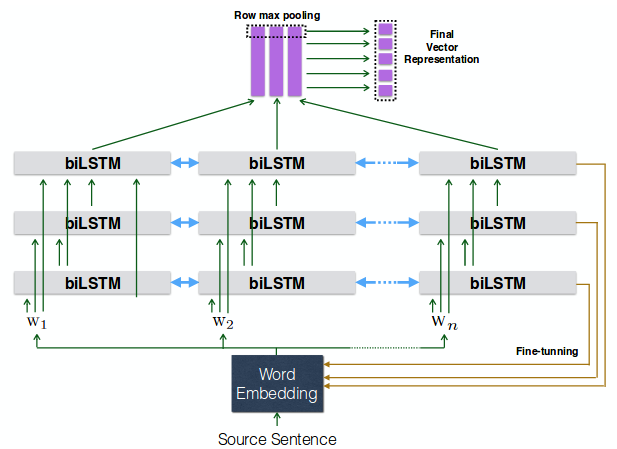
\includegraphics[totalheight=8cm]{fig/sentence_encoder_shortcut.png}
	\caption{The architecture of the sentence-encoding component within the Shortcut-Stacked-Encoder, taken from \cite{nie2017shortcut}.}
	\label{fig:sentence_emcoder_shortcut}
\end{figure}
Due to the arbitrary length of words in textual input a widely used strategy to encode variable length inputs to fixed length vectors using \ac{LSTM} \citep{hochreiter1997long} or the bidirectional variant \ac{biLSTM} \citep{graves2005framewise}. Essentially these components learn with the use of gates what information to keep and forget at a given point in time. By sequentially going through a sentence in one or two directions respectivly, are capable of exploiting word-order and take context into account.
\newline

The main difference of the Shortcut-Stacked Sentence-Encoder to typical approaches of a multi-layer \ac{biLSTM} model is that the input to the \ac{biLSTM} in a following layer is not only the output of the previous layer, but the output of \textit{all} previous layers, together with the word embeddings. In the first step, the embedding layer maps each word $\omega_i$ of the source sentence $(\omega_1, \omega_2, ..., \omega_n)$ to a $d$-dimensional word vector $w_i \in \mathbb{R}^d$. According to \cite{nie2017shortcut} we denote $x_t^i$ to be the input of the $i$th \ac{biLSTM} at timestep $t$. Naturally the input to the first layer are the word-embeddings itself, thus:
\begin{equation}
x_t^1 = w_t
\end{equation} 
In all \ac{biLSTM} with $i > 1$ the input is the concatenation of all intermediate inputs of previous layers at the timestep $t$ together with the initial word embeddings. Let $[]$ denote the vector concatenation and $h^i_t$ be the output of the $i$th \ac{biLSTM} at timestep $t$, this leads to:
\begin{equation}\label{eq:stacked_encoder_input}
x_t^i = [w_t, h_t^{i-1}, h_t^{i-2}, ... , h_t^1]
\end{equation}

Only the last \ac{biLSTM} layer is used to generate the final sentence representation. Assuming $m$ layers in total, $d_m$ to be the hidden state dimension of the last layer, that is defined as $H_m=(h_1^m, h_2^m, ..., h_n^m)$ the final sentence representation $v$ is obtained by applying row-max-ppoling over the last layer:
\begin{equation}
v = max(H^m)
\end{equation}
With each $h_i^m \in \mathbb{R}^{2d_m}$ and $H^m \in \mathbb{R}^{2d_m \times n}$ the resulting sentence vector $v \in \mathbb{R}^{2d_m}$ essentiallly captures the highest value of each dimension over all timesteps\footnote{$d_m$ is multiplicated by $2$ since the \ac{biLSTM} creates $d_m$ features for going through the sentence forwards and backwards repsectively.}.
\subsubsection{Classification}
A two-layer \ac{MLP} using ReLu as acticvation function and a final softmax-layer is used for the prediction. The input to the classifier $m$ is the concatention of the sentence representations $v_p$ and $v_h$ for $p$ and $h$ respectively together with the element-wise distance and the elementwise product, denoted as $\otimes$ of both representations:
\begin{equation}
m = [v_p, v_h, |v_p-v_h|, v_p \otimes v_h]
\end{equation}
Even thow a multi-layer \ac{MLP} theoretically would be able to learn the latter two features, \cite{mou2015natural} showed that this particular feature concatenation gives a performance gain for neural models for \ac{NLI}.
\subsubsection{Training}
For all our reimplementations using pytorch\footnote{\href{http://pytorch.org/}{http://pytorch.org/}} of the model we follow the parameters of the original paper of \cite{nie2017shortcut}. The model is trained using Adam \citep{kingma2014adam} parameter optimization, cross-entropy loss as objective function and minibatches of size 32. To avoid overfitting a dropout of 0.1 is applied on each layer of the \ac{MLP} and the accuracy is evaluated regulary on a different dataset than the train data, the development set, as it is common practive in machine learning. The final performance is estimated by evaluating the best model based on the accuracy on the development set on unseen hold-out data, the test set. 300-dimensional GloVe 840B pretrained word-embeddings \citep{pennington2014glove} are used and finetuned during training. Three additional word-vectors are added, one for unknown words, as well as one to indicate the start and one to indicate the end of a sentence. The learning rate starts with 0.0002 and is reduced by half every second iteration. We conduct our experiments with different re-implementations of this model, partly due to using fewer parameters by reducing the dimensionality of the components, partly due to changes within the original paper.
\subsubsection{Residual Encoder and Reimplementation Variants}
In a second version of the paper, \cite{nie2017shortcut} introduced the Residual Encoder, slightly adapting the way sentences are encoded. In order to create the input to the $i$th \ac{biLSTM} layer $x_t^i$ concatenation all previous outputs $(h_t^{i-1}, h_t^{i-2}, ... , h_t^1)$ together with $w_t$, naturally leads to a tremendous increase of parameters. By using residual connections, instead of concatenating all previous outputs, they are added up, thus equation (\ref{eq:stacked_encoder_input}) changes to
\begin{equation}
x_t^i = [w_t, h_t^{i-1} + h_t^{i-2} + ... + h_t^1]
\end{equation}
and reduces the parameter size.
\paragraph*{Implementation Variants}
We use the following implementations of the model. The performance comparison between the models based on SNLI\footnote{SNLI is a huge dataset for \ac{NLI} and will be explained in §\ref{sec:basics_datasets}}, is listed in Table \ref{table:reimplementation_performance} and do not differ tremendously from what \cite{gong2017natural} estimated to be the human performance on the same task.
\begin{table}[!htbp]
\begin{center}
\begin{tabular}{lccc}
\textbf{Model} & \textbf{SNLI train acc.} & \textbf{SNLI dev acc.} & \textbf{SNLI test acc.}\\
\toprule
Shortcut-Stacked Encoder\textsuperscript{$\dagger$} & 87.4\% & 85.2\% & 84.8\% \\
Shortcut-Stacked Encoder\textsuperscript{$\dagger\dagger$} & 89.4\% & 86.0\% & 85.4\% \\
Residual Encoder\textsuperscript{$\dagger$} & 91.1\% & 85.9\% & 85.8\% \\
Residual Encoder\textsuperscript{$\Diamond$} & 91.0\% & 87.0\% & 86.0\% \\
\midrule
Human Performance \citep{gong2017natural} & - & - & 87.7 \\
\bottomrule
\end{tabular}
\caption{Accuracy in percent of different implementations of the model from \cite{nie2017shortcut}, achieved on the SNLI dataset compared with human performance.}
\label{table:reimplementation_performance}
\end{center}
\end{table}
\begin{itemize}
\item We refer to Shortcut-Stacked Encoder\textsuperscript{$\dagger$} as the first re-implementation. This uses $256\times2$, $512\times2$ and $1024\times2$ dimensions for the three layers of the sentence encoding \ac{biLSTM} and $1600$ dimensions in the classifier \ac{MLP}.
\item We refer to Residual Encoder\textsuperscript{$\dagger$} when we use our own re-implementation with residual connections. The sentence-encoding \ac{biLSTM}s each have the dimensionality of $600\times2$ and the layers of the \ac{MLP} of $800$.
\item We refer to Residual Encoder\textsuperscript{$\Diamond$} when we use the final published version of \cite{nie2017shortcut} with their provided code\footnote{https://github.com/easonnie/ResEncoder}. This model has the same parameter sizes as Residual Encoder\textsuperscript{$\dagger$}.
\item We refer to the plain model name, when talking about the model structure in general.
\end{itemize}
